% !TeX spellcheck = en_US
\documentclass[a4paper]{scrartcl}

\usepackage[utf8]{inputenc}
\usepackage[english]{babel}
\usepackage[T1]{fontenc}
\usepackage{lmodern}
\usepackage{amsmath}
\usepackage{amssymb}
\usepackage{pdflscape}
\usepackage{geometry}
\usepackage{xcolor}
\usepackage{graphicx}
\usepackage{todonotes}
\setlength{\parindent}{0pt}

\usepackage{biblatex}
\addbibresource{references.bib}


%\geometry{a4paper, top=25mm, left=30mm, right=20mm, bottom=30mm,
%headsep=10mm, footskip=12mm}

\newcommand{\itab}[1]{\hspace{0em}\rlap{#1}}
\newcommand{\tab}[1]{\hspace{.2\textwidth}\rlap{#1}}
\newcommand{\asd}[1]{\textbf{#1}}

\title{Concepts for Digram types}
\author{Matthias Dürksen}
\date{\today}
 

\begin{document}
\maketitle

\section{Basic digram}\label{sec:motivation}

Everything as in~\cite{mattdk}.

The basic digram (Fig.~\ref{fig:basicDigram}) consists of two adjacent nodes and the edge that connects these nodes. Thus, two adjacent nodes and the incident edge can be replaced by one nonterminal symbol. Each node is assigned with an equivalence class.

\begin{figure}[h]
	\centering
	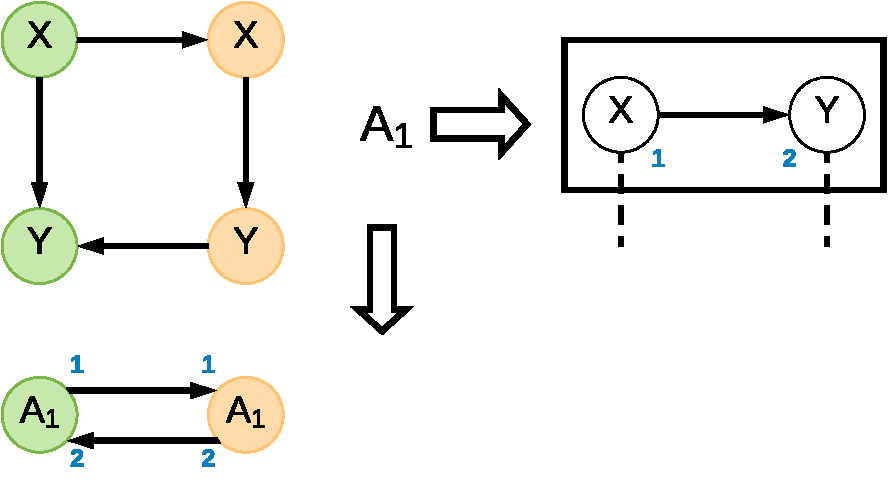
\includegraphics[width=0.6\textwidth]{img/basicDigram}
	\caption{Application of a replacement of a basic digam}
	\label{fig:basicDigram}
\end{figure}

\section{Adjacent digram}

Everything as in~\cite{mattdk}.

The adjacency digram (Fig.~\ref{fig:adjazenzDigram}) is formed by two nodes which both have a common adjacency node b. Thus, the adjacency digram contains the two nodes and the two edges that are incident to the node b. This digram can be replaced by a nonterminal and an edge from the nonterminal to the node b. Each inner node is assigned an equivalence class. Node b does not require an equivalence class.

\begin{figure}[h]
	\centering
	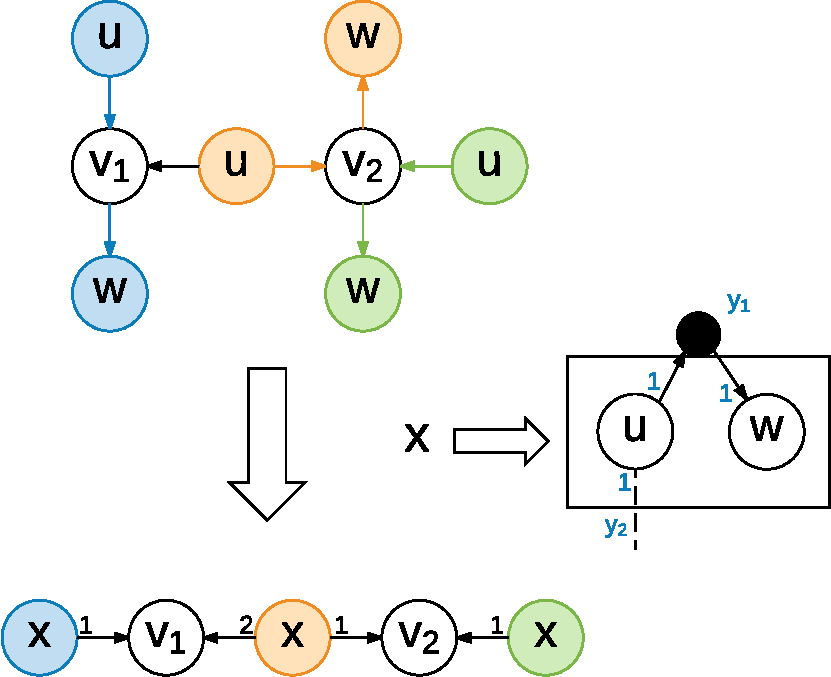
\includegraphics[width=0.5\textwidth]{img/adjazenzDigram}
	\caption{Application of a replacement of an adjacency digam}
	\label{fig:adjazenzDigram}
\end{figure}


\section{Node association digram}

The node assaciation digram (Fig.~\ref{fig:nodeAssociationDigram}) is a generalization of an adjacent digram.
This digram consists of two nodes, which are replaced in a substitution of an occurrence by a node. Each node is assigned with an equivalence class.
In this way, frequently occurring nodes are replaced by a node and these do not have to be adjacent. However, this replacement increases the number of incident nodes, since the new node unites the incident edges of the old nodes.

\begin{figure}[h]
	\centering
	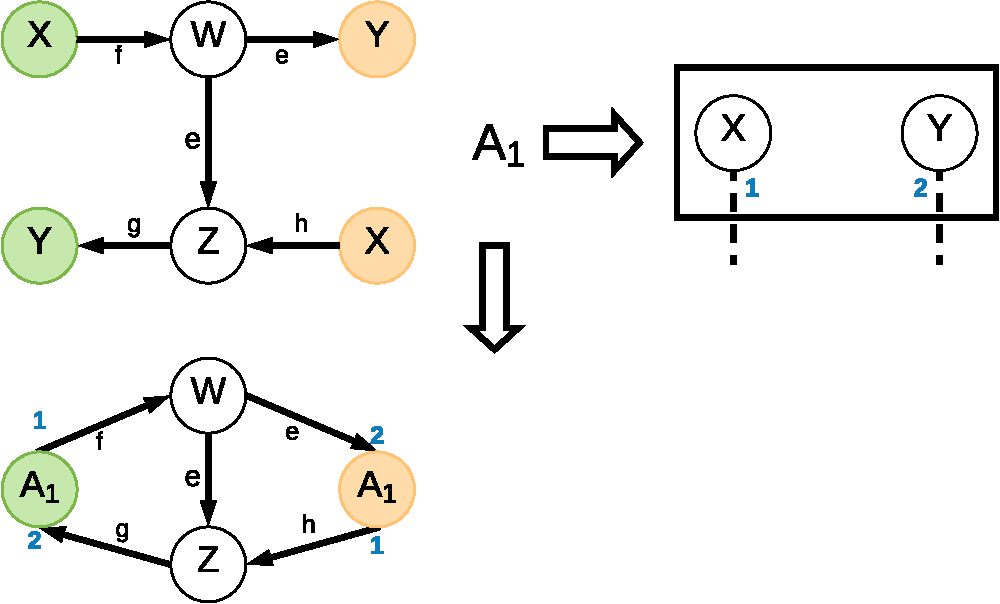
\includegraphics[width=0.5\textwidth]{img/nodeAssociationDigram}
	\caption{Application of a replacement of a node association digam}
	\label{fig:nodeAssociationDigram}
\end{figure}


\section{Clique digram}

The clique digram (Fig.~\ref{fig:cliqueDigram}) is a generalization of an adjazenz digram.
This clique digram consists of two nodes, which are strongly connected. The occurrences are replaced by a node. Each node is assigned an equivalence class. The digram can also be generated by applying basic digrams twice. The advantage of this digram rule is that the individual edges do not have to be stored in the digram rule, because the information is implicit present. If one of the two nodes is already a nonterminal, the other node should be adjacent to each inner node.

\begin{figure}[h]
	\centering
	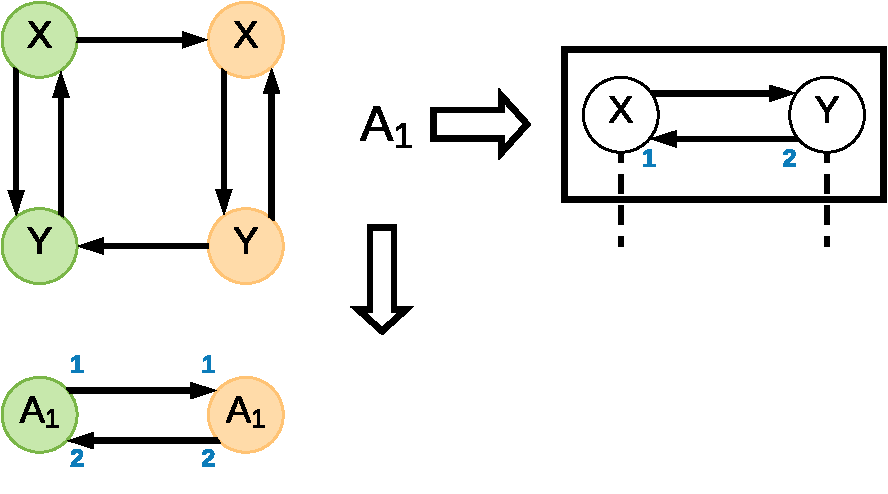
\includegraphics[width=0.5\textwidth]{img/cliqueDigram}
	\caption{Application of a replacement of a clique digam}
	\label{fig:cliqueDigram}
\end{figure}



\section{Basic edge digram}

The basic edge digram (Fig.~\ref{fig:basicEdgeDigram}) is the opposite of the basic digam.
Here, two edges and a node, where both edges are incident to the node, are replaced by one edge. The directions of the edges must be the same in all occurrences. If the node is already a nonterminal, you have to save which edge goes into which equivalence class.

\begin{figure}[h]
	\centering
	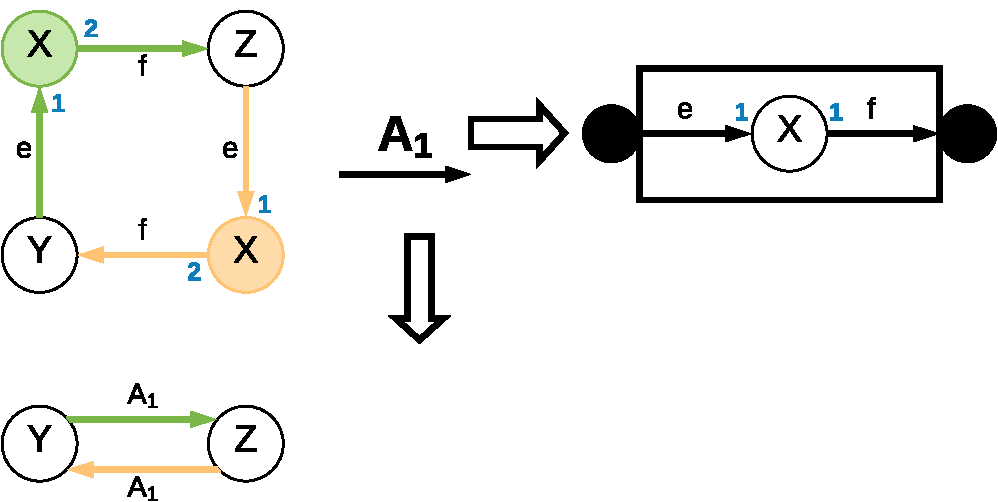
\includegraphics[width=0.7\textwidth]{img/basicEdgeDigram}
	\caption{Application of a replacement of a basic Edge digam}
	\label{fig:basicEdgeDigram}
\end{figure}




\pagebreak
\printbibliography







\end{document}